\documentclass[aspectratio=169,xcolor=dvipsnames]{beamer}
\usetheme{Simple}
\usepackage[T1]{fontenc}
\usepackage[utf8]{inputenc}
\usepackage[english]{babel}
\usepackage{graphicx}
\usepackage{booktabs}
\usepackage{array}
\usepackage{ragged2e}
\newcolumntype{L}[1]{>{\RaggedRight\arraybackslash}p{#1}}
\usepackage{xcolor}
\usepackage{hyperref}

\definecolor{CyberRed}{HTML}{B42332}
\definecolor{CyberBurgundy}{HTML}{7F1D1D}
\definecolor{CyberLight}{HTML}{FCE8EA}
\definecolor{CyberText}{HTML}{292525}
\setbeamercolor{normal text}{fg=CyberText,bg=white}
\setbeamercolor{structure}{fg=CyberRed}
\setbeamercolor{title}{fg=white}
\setbeamercolor{subtitle}{fg=white}
\setbeamercolor{frametitle}{fg=CyberBurgundy,bg=white}
\setbeamercolor{section in toc}{fg=CyberBurgundy}
\setbeamercolor{item}{fg=CyberRed}
\setbeamercolor{subitem}{fg=CyberRed}
\setbeamercolor{enumerate item}{fg=CyberRed}
\setbeamercolor{alerted text}{fg=CyberRed}
\setbeamercolor{block title}{fg=white,bg=CyberBurgundy}
\setbeamercolor{block body}{fg=CyberText,bg=CyberLight}
\setbeamercolor{block title alerted}{fg=white,bg=CyberRed}
\setbeamercolor{block body alerted}{fg=CyberText,bg=CyberLight}
\setbeamercolor{block title example}{fg=white,bg=CyberBurgundy}
\setbeamercolor{block body example}{fg=CyberText,bg=CyberLight}
\setbeamercolor{palette primary}{fg=white,bg=CyberRed}
\setbeamercolor{palette secondary}{fg=white,bg=CyberBurgundy}
\setbeamercolor{palette tertiary}{fg=white,bg=CyberBurgundy}
\setbeamercolor{footline}{fg=CyberBurgundy,bg=white}
\setbeamercolor{navigation symbols}{fg=CyberRed}
\hypersetup{colorlinks=true,urlcolor=CyberRed,linkcolor=CyberBurgundy,citecolor=CyberRed}

% EDIT THE FIELDS BELOW.
\title[Azure AI -- Module 1]{Microsoft Azure AI -- Module 1}
\subtitle{Microsoft Azure -- Practical Approach \\ Azure Virtual Machines as an IaaS solution}
\author[Student / team]{Filip Kłos, Szymon Kaczmarek, Krzysztof Szczepaniak, Jakub Rybczyński, Dorian Koehler}
\institute[SUT]{Faculty of Applied Mathematics\\Silesian University of Technology}
\date{\today}

\begin{document}
\begin{frame}
\titlepage
\end{frame}
\begin{frame}{Presentation outline}
\tableofcontents
\end{frame}
\section{Introduction}
\begin{frame}{Selected Azure topic and objectives}
\begin{itemize}
\item \textbf{Selected topic:} Azure Virtual Machines (IaaS)
\item \textbf{Problem context:} A team needs a Linux environment where it can install custom runtimes, configure the OS, and run software that is not easily packaged for a PaaS platform.
\item \textbf{Why Azure VMs:} They provide the highest degree of control over the VM and its operating system compared with other Azure compute options
\item \textbf{What will be presented:} VM concepts, portal configuration choices, a practical deployment/inspection, observed results, and cost/security trade-offs.
\item \textbf{Note:} Azure VMs free you from buying physical hardware, but they do not free you from OS maintenance, patching and software installation remain your responsibility.
\end{itemize}
\end{frame}
\section{Cloud concepts}
\begin{frame}{Cloud foundations and terminology}
	\begin{itemize}
		\item \textbf{IaaS (Infrastructure as a service)} - You rent compute, manage the OS, runtime, and applications.
		\item \textbf{PaaS (Platform as a service)} - You rent service, don't manage underlying OS
		\item \textbf{Where VMs fit} - Azure VMs are one of several on-demand, scalable compute resource types in Azure
		\item \textbf{Prerequisites} - An Azure subscription, a resource group, a region, permission to create resources.
		\item \textbf{Billing boundary} - The subscription defines billing and access; the resource group collects related resources.
	\end{itemize}
\end{frame}
\section{Azure exploration}
\begin{frame}{Selected service: overview}
\begin{itemize}
\item \textbf{Purpose of Azure VMs} - On-demand, scalable compute with virtualization, without purchasing physical hardware.
\item \textbf{Common use cases} - Development and testing, cloud applications with variable demand, and extending an on-premises network into Azure.
\item \textbf{Key configuration choices}
 \begin{itemize}
 	\item Subscription
 	\item Region and resource group
 	\item VM name
 	\item VM image
 	\item VM architecture
 	\item VM size/family
 	\item Authentication
 	\item Inbound port rules
 \end{itemize}
 \item \textbf{Where to find it} Azure portal → Create a resource → search Virtual machine.
\end{itemize}
\end{frame}
\begin{frame}{Azure VM families}
	\textbf{The first cost/performance decision}
	
	\vspace{0.2cm}
	Azure groups VM sizes into \textbf{families} by CPU-to-memory ratio and
	specialised hardware. The wrong family causes overspending
	or underperformance
	
	\vspace{0.3cm}
	\textbf{The name encodes the specification}
	
	\vspace{0.1cm}
	{\footnotesize
		\begin{center}
			\begin{tabular}{@{}ll@{}}
				\toprule
				\textbf{Part} & \textbf{Meaning (example)} \\
				\midrule
				\textbf{D}  & Family: General purpose \\
				\textbf{C}  & Subfamiily \\
				\textbf{a}  & CPU info \\
				\textbf{d}  & Storage \\
				\textbf{s}  & Premium storage \\
				\textbf{v5} & 5th hardware generation \\
				\bottomrule
			\end{tabular}
		\end{center}
	}
\end{frame}
\begin{frame}[shrink=10]{Core VM families}
	\centering
	\renewcommand{\arraystretch}{1.4}
	\setlength{\tabcolsep}{4pt}
	\small
	
	\begin{tabular}{@{} L{1.6cm} L{2.2cm} L{2.6cm} L{3.8cm} L{3.2cm} @{}}
		\toprule
		\textbf{Family} & \textbf{Focus} & \textbf{Approx.\ profile} & \textbf{Best for} & \textbf{Cost note} \\
		\midrule
		\textbf{B-series} & Burstable
		& Baseline + CPU credits
		& Dev/test, low-traffic servers, occasional spikes
		& Lowest for idle-heavy use; throttled when credits end \\
		\addlinespace
		\textbf{D-series} & General purpose
		& Balanced ($\sim$4\,GB/vCPU)
		& Web/app servers, microservices
		& Default baseline; steady performance \\
		\addlinespace
		\textbf{E-series} & Memory optimised
		& High RAM ($\sim$8\,GB/vCPU)
		& In-memory DBs, caches, analytics
		& Higher cost/vCPU; pay for RAM \\
		\addlinespace
		\textbf{F-series} & Compute optimised
		& High CPU ($\sim$2\,GB/vCPU)
		& Batch, CI/CD, CPU-bound tiers
		& Cheaper than D for pure compute \\
		\addlinespace
		\textbf{L-series} & Storage optimised
		& High IOPS, local NVMe
		& Big Data, NoSQL, warehousing
		& Maximises disk, not CPU/RAM \\
		\addlinespace
		\textbf{N-series} & GPU accelerated
		& Specialised GPU
		& AI training/inference, rendering
		& Highest tier; GPU choice critical \\
		\bottomrule
	\end{tabular}
\end{frame}
\begin{frame}[shrink=15]{B-series in focus: the credit model and a decision path}
	\begin{columns}[T]
		\begin{column}{0.48\textwidth}
			\vspace{0.2cm}
			\textbf{\large How burstable billing works}
			
			\vspace{0.3cm}
			\begin{itemize}
				\setlength{\itemsep}{0.8em}
				\item B-series uses \textbf{CPU credits} for performance.
				\item Below baseline $\rightarrow$ \textbf{accumulate} credits.
				\item Need more power $\rightarrow$ \textbf{burst} up to 100\% vCPU.
				\item Credits exhausted $\rightarrow$ \textbf{throttled} to baseline until they recover.
			\end{itemize}
			
			\vspace{0.4cm}
			\begin{exampleblock}{When to avoid B-series}
				Sustained high CPU (e.g.\ 80\ for hours) exhausts credits and throttles. Use \textbf{D} or \textbf{F} for steady load.
			\end{exampleblock}
		\end{column}
		
		\begin{column}{0.48\textwidth}
			\vspace{0.2cm}
			\textbf{\large A simple decision path}
			
			\vspace{0.3cm}
			\begin{itemize}
				\setlength{\itemsep}{0.8em}
				\item \textbf{Spiky/idle CPU?} \\
				$\hookrightarrow$ Choose \textbf{B-series} (dev/test)
				
				\item \textbf{Steady general workload?} \\
				$\hookrightarrow$ Choose \textbf{D-series} (web/app)
				
				\item \textbf{Needs massive RAM?} \\
				$\hookrightarrow$ Choose \textbf{E-series} (in-memory DB)
				
				\item \textbf{CPU-heavy, low RAM?} \\
				$\hookrightarrow$ Choose \textbf{F-series} (batch, CI)
				
				\item \textbf{Needs high disk IOPS?} \\
				$\hookrightarrow$ Choose \textbf{L-series} (Big Data)
				
				\item \textbf{Needs GPU?} \\
				$\hookrightarrow$ Choose \textbf{N-series} (AI)
			\end{itemize}
		\end{column}
		
	\end{columns}
\end{frame}
\begin{frame}{Practical demonstration}
\begin{itemize}
\item To create a new Azure Virtual Machine, enter \textit{virtual machines} in search bar.
\item Under \textbf{Services}, select \textbf{Virtual Machines}.
\item In the \textbf{Virtual machines} page, select \textbf{Create} from the menu at the top of the page and then select \textbf{Virtual machine} from the drop-down. The \textbf{Create a virtual machine} page opens.
\item Under \textbf{Instance details}, enter \textit{myVM} for the Virtual machine name and choose \textit{Windows Server 2022 Datacenter: Azure Edition - x64 Gen 2} for the Image. The page will fill in the other fields with defaults and use the VM name to create similar names for the other resources that are needed.
\end{itemize}
\end{frame}
\begin{frame}{Practical demonstration}
	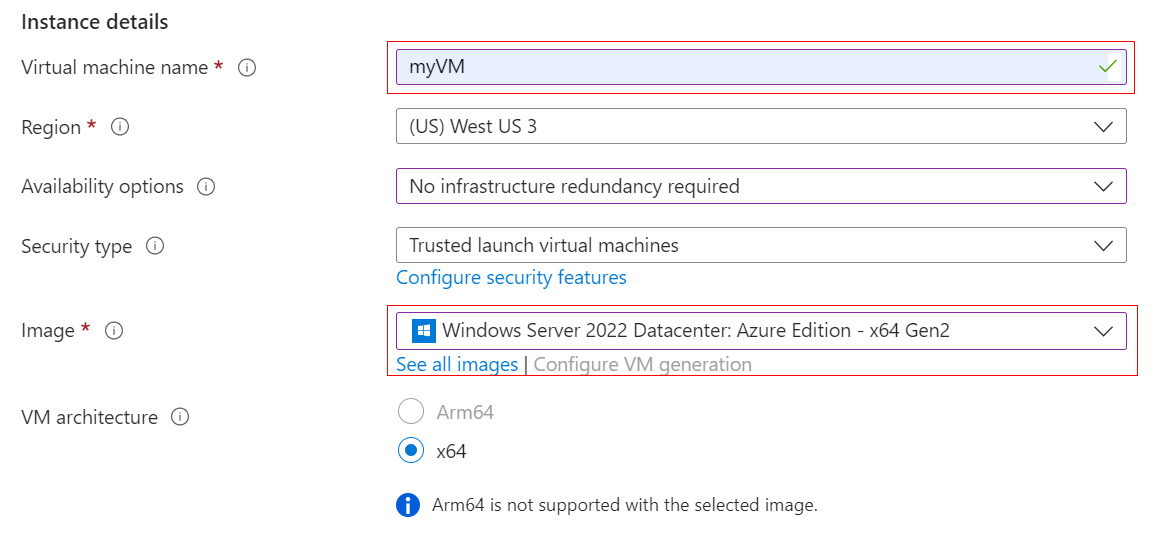
\includegraphics[width=\textwidth]{img/1.png}
\end{frame}
\begin{frame}{Practical demonstration}
\begin{itemize}
	\item Under \textbf{Administrator account}, provide a username, such as \textit{azureuser} and a password. The password must be at least 12 characters long and meet the defined complexity requirements.
\end{itemize}
	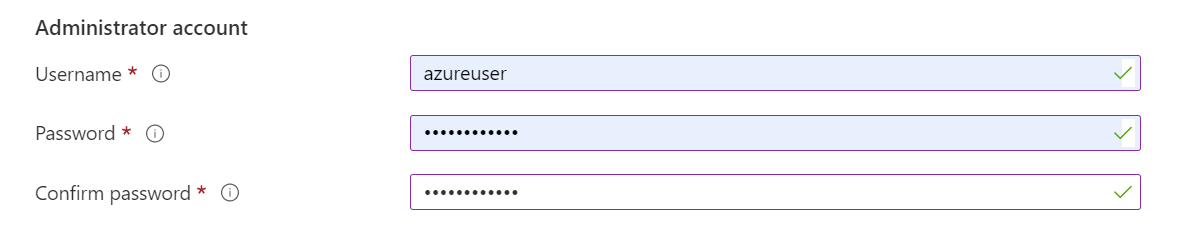
\includegraphics[width=\textwidth]{img/2.png}
\end{frame}
\begin{frame}{Practical demonstration}
	\begin{itemize}
		\item Under \textbf{Inbound port rules}, choose \textbf{Allow selected ports} and then select \textbf{RDP (3389)} and \textbf{HTTP (80)} from the drop-down.
	\end{itemize}
	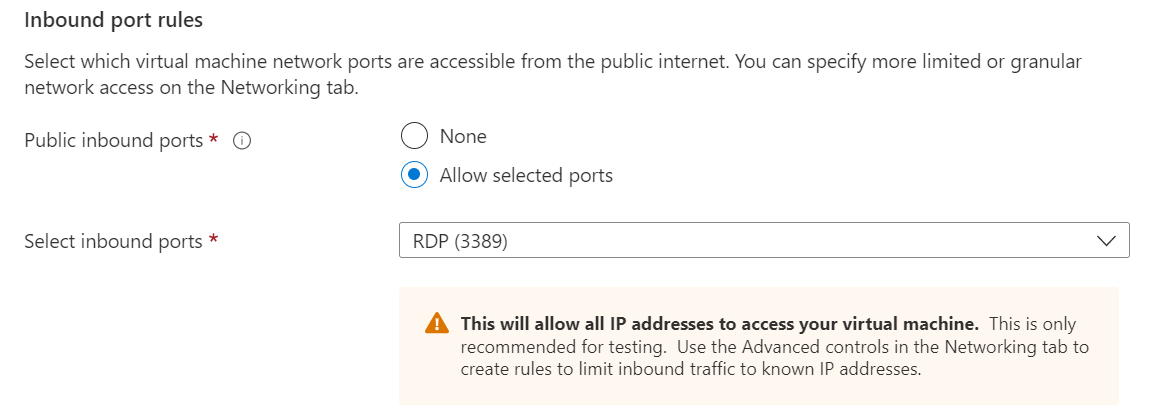
\includegraphics[width=\textwidth]{img/3.png}
\end{frame}
\begin{frame}{Practical demonstration}
	\begin{itemize}
		\item At the top of the page, select the \textbf{Management} tab.
		\item In the \textbf{Auto-shutdown} section, select the \textbf{Enable auto-shutdown} option.
		\item Select a \textbf{Shutdown time} and the \textbf{Time zone} to use (UTC is the default). Optionally you can choose to be notified by e-mail before the shutdown.
	\end{itemize}
\end{frame}
\begin{frame}{Practical demonstration}
	\begin{itemize}
		\item Leave the remaining defaults and then select the \textbf{Review + create} button at the bottom of the page.
	\end{itemize}
	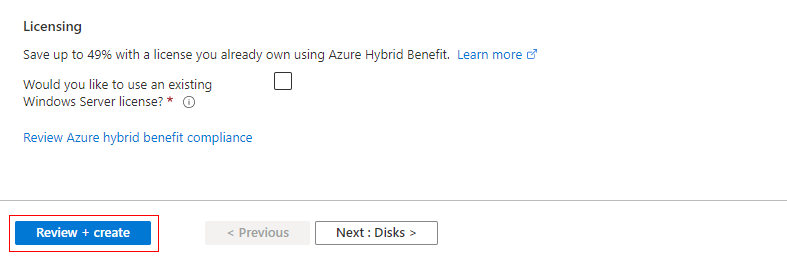
\includegraphics[width=\textwidth]{img/4.png}
\end{frame}
\begin{frame}{Practical demonstration}
	\begin{itemize}
		\item After validation runs, select the \textbf{Create} button at the bottom of the page.
	\end{itemize}
	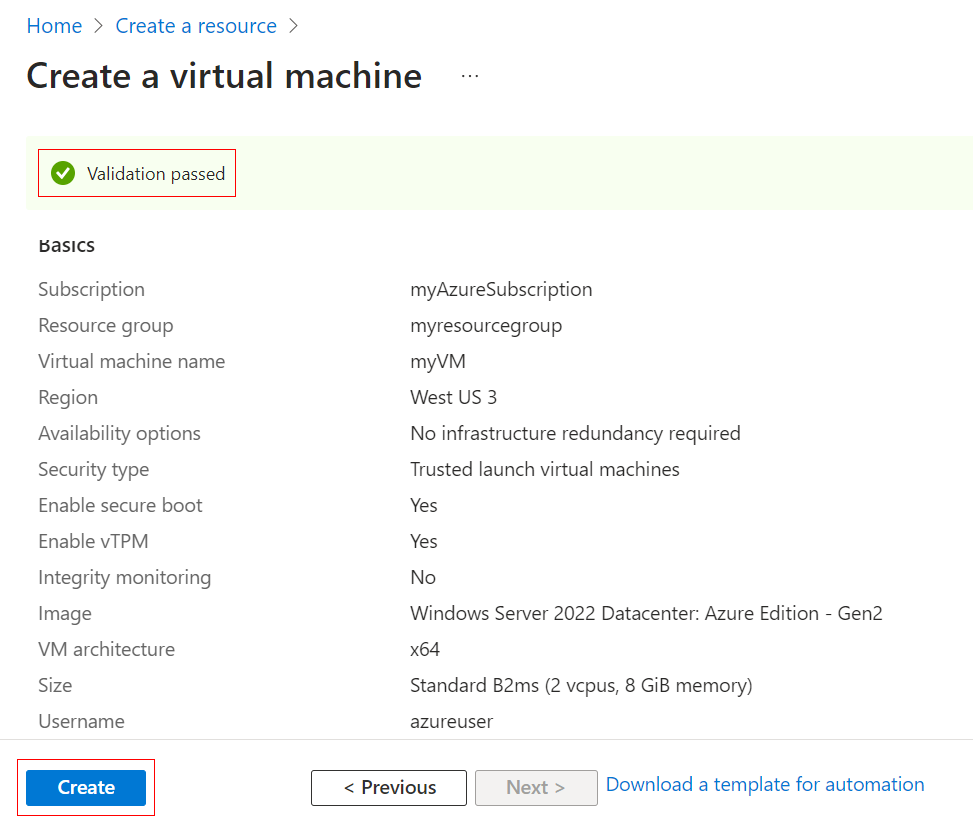
\includegraphics[width=\textwidth]{img/5.png}
\end{frame}
\begin{frame}{Practical demonstration}
	\begin{itemize}
		\item After deployment is complete, select \textbf{Go to resource}.
	\end{itemize}
	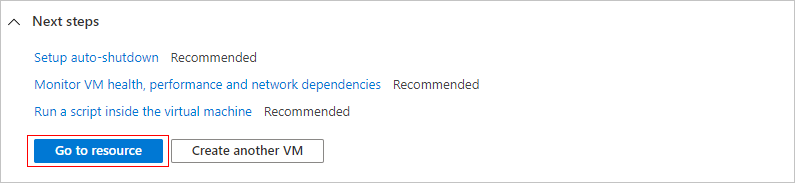
\includegraphics[width=\textwidth]{img/6.png}
\end{frame}
\begin{frame}{Practical demonstration}
	Connect to virtual machine
	\begin{itemize}
		\item On the overview page for your virtual machine, select \textbf{Connect} and then select \textbf{Connect} again from the drop-down.
		\item In the \textbf{Native RDP} page, select the \textbf{Check access} button to make sure port 3389 is available.
		\item Select \textbf{Download RDP file} to download the connection file to your computer.
		\item Open the downloaded RDP file and click \textbf{Connect} when prompted.
		\item You may receive a certificate warning during the sign-in process. Click \textbf{Yes} or \textbf{Continue} to create the connection.
	\end{itemize}
\end{frame}
\begin{frame}{Screenshots and observations}
\begin{itemize}
	\item Insert a screenshot or a simple diagram illustrating the selected service.
	\item Describe what the screenshot demonstrates.
	\item Identify one meaningful observation from the exploration.
	\item Explain what could be tested or explored next.
\end{itemize}
\end{frame}
\section{Results}
\begin{frame}{Key findings}
\begin{itemize}
    \item \textbf{Flexibility and control}
    \begin{itemize}
        \item Azure VMs provide full control over the operating system,
        installed software and runtime environment.
        \item They support different operating systems, architectures
        and workload requirements.
    \end{itemize}

    \item \textbf{Scalability and availability}
    \begin{itemize}
        \item VM sizes can be selected according to CPU, memory and
        storage requirements.
        \item Resources can be scaled up or down as workload demands change.
    \end{itemize}

    \item \textbf{Cost optimisation}
    \begin{itemize}
        \item Different VM families allow optimisation for specific workloads.
        \item B-series VMs can reduce costs for workloads with variable CPU usage.
        \item Auto-shutdown helps avoid unnecessary compute costs.
    \end{itemize}

    \item \textbf{Cloud integration}
    \begin{itemize}
        \item VMs can be integrated with other Azure services,
        networks and storage solutions.
    \end{itemize}
\end{itemize}
\end{frame}

\begin{frame}{Practical advantages and limitations}
\begin{columns}[T]
    \begin{column}{0.48\textwidth}
        \textbf{\large Advantages}
        \begin{itemize}
            \item No need to purchase or maintain physical hardware.
            \item Full control over the operating system.
            \item Support for custom software and configurations.
            \item Flexible resource selection.
            \item Integration with the Azure ecosystem.
            \item Ability to automate deployment and management.
        \end{itemize}
    \end{column}

    \begin{column}{0.48\textwidth}
        \textbf{\large Limitations}
        \begin{itemize}
            \item Operating system updates and security remain the user's responsibility.
            \item Costs can increase if resources are not managed properly.
            \item Incorrect VM sizing can cause poor performance or overspending.
            \item Network and access configuration require attention.
            \item B-series performance depends on available CPU credits.
        \end{itemize}
    \end{column}
\end{columns}
\end{frame}


\begin{frame}{Lessons learned}
\begin{itemize}
    \item \textbf{Choosing the right VM size matters}
    \begin{itemize}
        \item VM selection should be based on actual workload requirements,
        not simply the highest available specifications.
    \end{itemize}

    \item \textbf{Security must be considered from the beginning}
    \begin{itemize}
        \item Only necessary inbound ports should be exposed.
        \item Strong authentication and regular security updates are essential.
    \end{itemize}

    \item \textbf{Cost management is important}
    \begin{itemize}
        \item Auto-shutdown can prevent unnecessary spending.
        \item VM deallocation should be considered when resources are no longer needed.
    \end{itemize}

    \item \textbf{IaaS requires more administration}
    \begin{itemize}
        \item Azure manages the underlying infrastructure,
        but users remain responsible for the guest operating system.
    \end{itemize}
\end{itemize}

\vspace{0.3cm}
\begin{block}{Main takeaway}
Azure Virtual Machines offer flexibility and control,
but efficient usage requires proper sizing, security
configuration and continuous cost management.
\end{block}
\end{frame}

\section{Conclusions and sources}
\begin{frame}{Conclusions}
\begin{enumerate}
\item Summarize the most important findings or project results.
\item Explain how the selected Azure services supported the work.
\item Discuss practical limitations and lessons learned.
\item Recommend feasible next steps.
\end{enumerate}
\end{frame}
\begin{frame}{References and resources}
\small
\begin{thebibliography}{9}
\bibitem{azure} Microsoft Learn, \emph{Microsoft Azure documentation}, \url{https://learn.microsoft.com/en-us/azure/}.
\bibitem{ai} Microsoft Learn, \emph{Azure AI services documentation}, \url{https://learn.microsoft.com/en-us/azure/ai-services/}.
\bibitem{paas} Microsoft \url{https://azure.microsoft.com/en-us/resources/cloud-computing-dictionary/what-is-paas}
\bibitem{iaas} Microsoft \url{https://azure.microsoft.com/en-us/resources/cloud-computing-dictionary/what-is-iaas/}
\bibitem{vmsize} Microsoft \url{https://learn.microsoft.com/en-us/azure/virtual-machines/sizes/overview}
\bibitem{bcpu} \url{https://learn.microsoft.com/en-us/azure/virtual-machines/sizes/b-series-cpu-credit-model}
\bibitem{other} Add the sources actually used in the presentation and project.
\end{thebibliography}
\end{frame}
\begin{frame}{Questions and discussion}
\centering
{\LARGE\bfseries Questions?}
\vspace{0.6cm}

{\large We welcome your questions and feedback.}
\end{frame}
\begin{frame}[plain]
\centering
{\Huge\bfseries Thank you!}
\end{frame}
\end{document}
